\TransitionFrame{modellazione del robot}

\begin{frame}{Modellazione}
\begin{columns}

\begin{column}{0.5\textwidth}
\begin{itemize}
    \item<1-> modello \textcolor{yellow}{discreto}
    \begin{itemize}
        \item<2-> approssimano un manipolatore continuo
    \end{itemize}
    \item<3-> numero $T$ arbitrario di link rigidi
    \item<4-> ogni link ha lunghezza $\ell_i$
    \begin{itemize}
        \item<5-> $N$ link con lunghezza $\ell_i$ grande per la parte prossimale
        \item<6-> $M$ link con lunghezza $\ell_j < \ell_i$ per la parte distale
        \item<6-> $T=N+M$
    \end{itemize}
    \item<7-> ogni giunto è sferico
    \begin{itemize}
        \item<8-> due giunti separati
        \item<9-> uno ruota sul proprio asse $x$
        \item<10-> uno ruota sul proprio asse $y$
    \end{itemize}
\end{itemize}
\end{column}

\begin{column}{0.6\textwidth}
\begin{center}
\only<1-6>{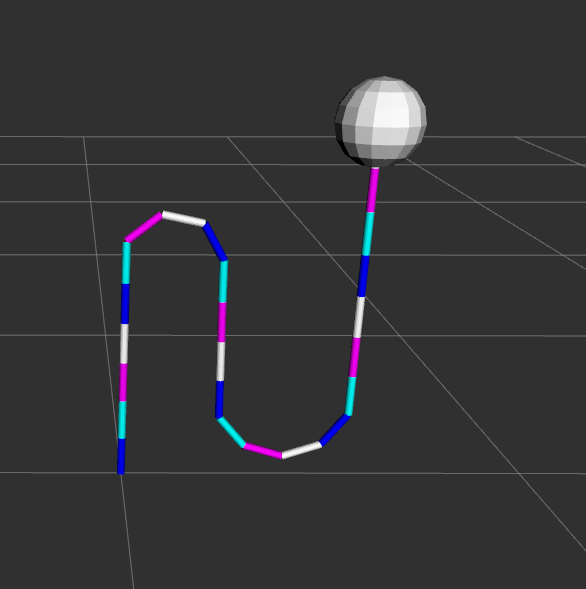
\includegraphics[height=0.7\textheight]{slide/img_modellazione/manipolatore-32-48.png}}
\only<7-10>{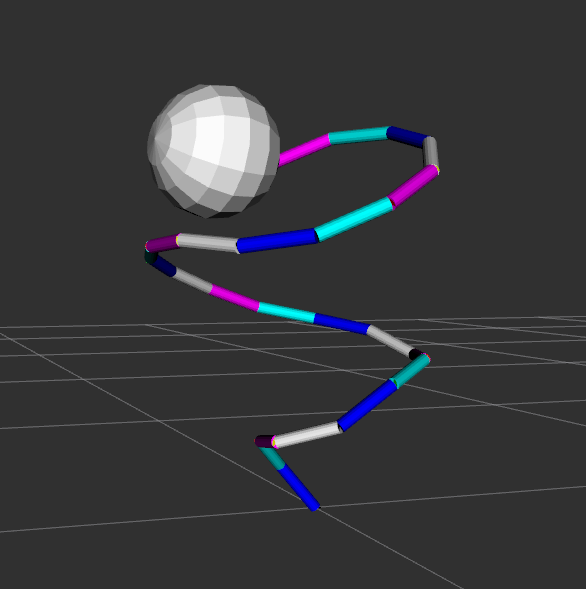
\includegraphics[height=0.7\textheight]{slide/img_modellazione/manipolatore-29-36.png}}
\end{center}
\end{column}
\end{columns}

\note{
Parte pratica \# 1: proporre modellazione manipolatori. 

Utilizzo modello rigid link, numero discreto di segmenti rigidi approssima con precisione arbitraria ogni manipolatore continuo. 

La lunghezza di ogni link non è necessariamente uguale $\to$ parte distale e prossimale.

Il giunto tra due link è sferico, viene modellato attraverso due giunti separati, uno che ruota intorno l'asse x ed uno intorno ad $y$. 
}

\end{frame}


\begin{frame}{Spazio di raggiungibilità}
\begin{columns}
\begin{column}{0.5\textwidth}
\begin{itemize}
    \item<1-> calcolo dello spazio di raggiungibilità
    \begin{itemize}
        \item<2-> semisfera
        \item<3-> raggio $r = \sum_{i = 1}^n \ell_i$
    \end{itemize}
\end{itemize}
\end{column}
\begin{column}{0.8\textwidth}
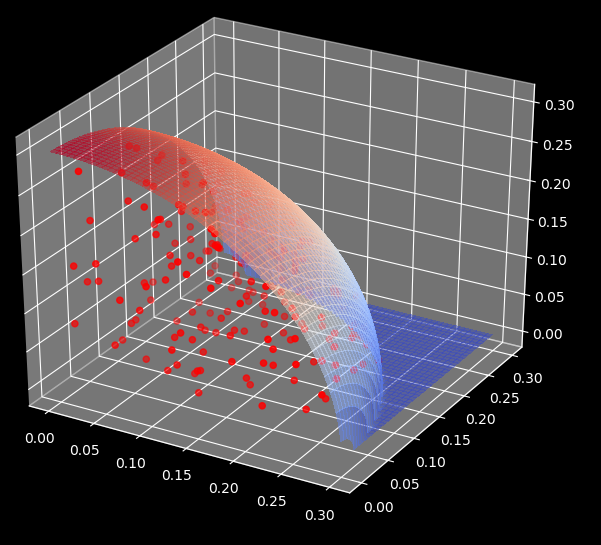
\includegraphics[width=0.7\textwidth]{slide/img_modellazione/spazio_raggiungibilita_red.png}
\end{column}
\end{columns}

\note{
Lo spazio di raggiungibilità del manipolatore è una semisfera di raggio pari alla somma delle lunghezze dei segmenti. 

L'end-effector deve essere quindi in grado di raggiungere i punti rossi del grafico. 
}

\end{frame}